 \documentclass[answers]{exam}
\usepackage{xeCJK}
\newif\ifanswers
% REMEMBER TO COMMENT OUT BEFORE GIVING TO PRETESTERS
\answerstrue %comment out to hide answers

\usepackage{fontspec}
\newfontfamily{\cherokeefam}{FreeSerif}

\newfontfamily{\monofam}{Latin Modern Mono}
\usepackage{lastpage} % Required to determine the last page for the footer
\usepackage{extramarks} % Required for headers and footers
\usepackage[usenames,dvipsnames]{color} % Required for custom colors
\usepackage{graphicx} % Required to insert images
\usepackage{listings} % Required for insertion of code
\usepackage{courier} % Required for the courier font
\usepackage{lipsum} % Used for inserting dummy 'Lorem ipsum' text into the template
\usepackage{enumerate}
\usepackage{subfigure}
\usepackage{booktabs}
\usepackage{amsmath, amsthm, amssymb}
\usepackage{hyperref}
\usepackage{datetime}
\settimeformat{ampmtime}
\usepackage{caption}

\usepackage{tikz}
\usetikzlibrary{positioning,patterns,fit,calc}
% Margins
\topmargin=-0.45in
\evensidemargin=0in
\oddsidemargin=0in
\textwidth=6.5in
\textheight=9.0in
\headsep=0.25in

\linespread{1.1} % Line spacing

\pagestyle{headandfoot}
\runningheadrule{}
\firstpageheader{CS 224n Spring 2024}{Assignment 3}{}
\runningheader{CS 224n Spring 2024} {Assignment 3} {Page \thepage\ of \numpages}
\firstpagefooter{}{}{} \runningfooter{}{}{}

\setlength\parindent{0pt} % Removes all indentation from paragraphs

%----------------------------------------------------------------------------------------
%	CODE INCLUSION CONFIGURATION
%----------------------------------------------------------------------------------------
\lstloadlanguages{bash}
\lstset{language=bash,
        frame=none, % Single frame around code
        basicstyle=\monofam, % Use small true type font
}

\usepackage{hyperref}
\hypersetup{
    colorlinks=true,
    linkcolor=blue,
    filecolor=magenta,      
    urlcolor=blue,
}
%----------------------------------------------------------------------------------------
%	NAME AND CLASS SECTION
%----------------------------------------------------------------------------------------

\newcommand{\hmwkTitle}{Assignment \#3} % Assignment title
\newcommand{\hmwkClass}{CS\ 224n Spring 2024} % Course/class
\newcommand{\hmwkAuthorName}{} % Author name
\newcommand{\ifans}[1]{\ifanswers \color{red} \vspace{5mm} \textbf{Solution: } #1 \color{black} \vspace{5mm} \fi}
\newcommand{\TODO}[1]{\color{magenta} \textbf{TODO:} #1 \color{black}}

\input std-macros
\input macros

%----------------------------------------------------------------------------------------
%	TITLE PAGE
%----------------------------------------------------------------------------------------
\qformat{\Large\bfseries\thequestion{}. \thequestiontitle{} (\thepoints{})\hfill}

\title{
\vspace{-1in}
\textmd{\textbf{\hmwkClass:\ \hmwkTitle} \\ \hmwkAuthorName}
}
\author{}
%\date{\textit{\small Updated \today\ at \currenttime}} % Insert date here if you want it to appear below your name
\date{}

\setcounter{section}{0} % one-indexing

\begin{document}

\maketitle
\vspace{-.5in}
\textbf{Due Date: April 30th, Tuesday, 4:30 PM PST.}


This assignment is split into two sections: \textit{Neural Machine Translation with RNNs} and \textit{Analyzing NMT Systems}. The first is primarily coding and implementation focused, whereas the second entirely consists of written, analysis questions. If you get stuck on the first section, you can always work on the second as the two sections are independent of each other. Note that the NMT system is more complicated than the neural networks we have previously constructed within this class and takes about \textbf{2 hours to train on a GPU}. Thus, we strongly recommend you get started early with this assignment. Finally, the notation and implementation of the NMT system is a bit tricky, so if you ever get stuck along the way, please come to Office Hours so that the TAs can support you. \newline

\begin{questions}
    \input q1
    \input q2
\end{questions}

\Large{\textbf{Submission Instructions}}

\normalsize
You shall submit this assignment on GradeScope as two submissions -- one for ``Assignment 3 [coding]" and another for `Assignment 3 [written]":
\begin{enumerate}
    \item Run the \texttt{collect\_submission.sh} script on the cloud VM to produce your \texttt{assignment3.zip} file. See \emph{How to Download the Gradescope Submission Package from Your Cloud VM} in the GCP How-to Appendix.
    \item Upload your \texttt{assignment3.zip} file to GradeScope to ``Assignment 3 [coding]".
    \item Upload your written solutions to GradeScope to ``Assignment 3 [written]". When you submit your assignment, make sure to tag all the pages for each problem according to Gradescope's submission directions. Points will be deducted if the submission is not correctly tagged.
\end{enumerate}

\newpage
\clearpage

\Large{\textbf{Appendix: GCP How-to}}\\
\normalsize
\paragraph{How to Obtain SSH connection info}
After following the instructions in the \href{https://docs.google.com/document/d/1FLx0CXIn-SoExxKM1efC-E-6iBjUR4uEnpGnfemMMR0/edit?pli=1#heading=h.4tqnggp12z76}{GCP Guide for CS224n}, your Gloogle Cloud Compute Engine dashboard should look like Fig \ref{fig:gcloud-compute-dashboard}. Click on the arrow button near SSH and select \textit{View gcloud command} as shown in the figure. What you will get looks like the following. Make a note of the zone, the machine name, and the project name which in the example are respectively \texttt{us-west4-b}, \texttt{nvidia-gpu-optimized-vmi-1-vm} and \texttt{grand-hangar-420500}. \textbf{Yours will be different!}

\begin{lstlisting}[
    breaklines=true,
    postbreak=\mbox{\textcolor{red}{$\hookrightarrow$}\space},
]
gcloud compute ssh --zone "us-west4-b" "nvidia-gpu-optimized-vmi-1-vm"  --project "grand-hangar-420500"
\end{lstlisting}

\begin{figure}[h]
    \centering
    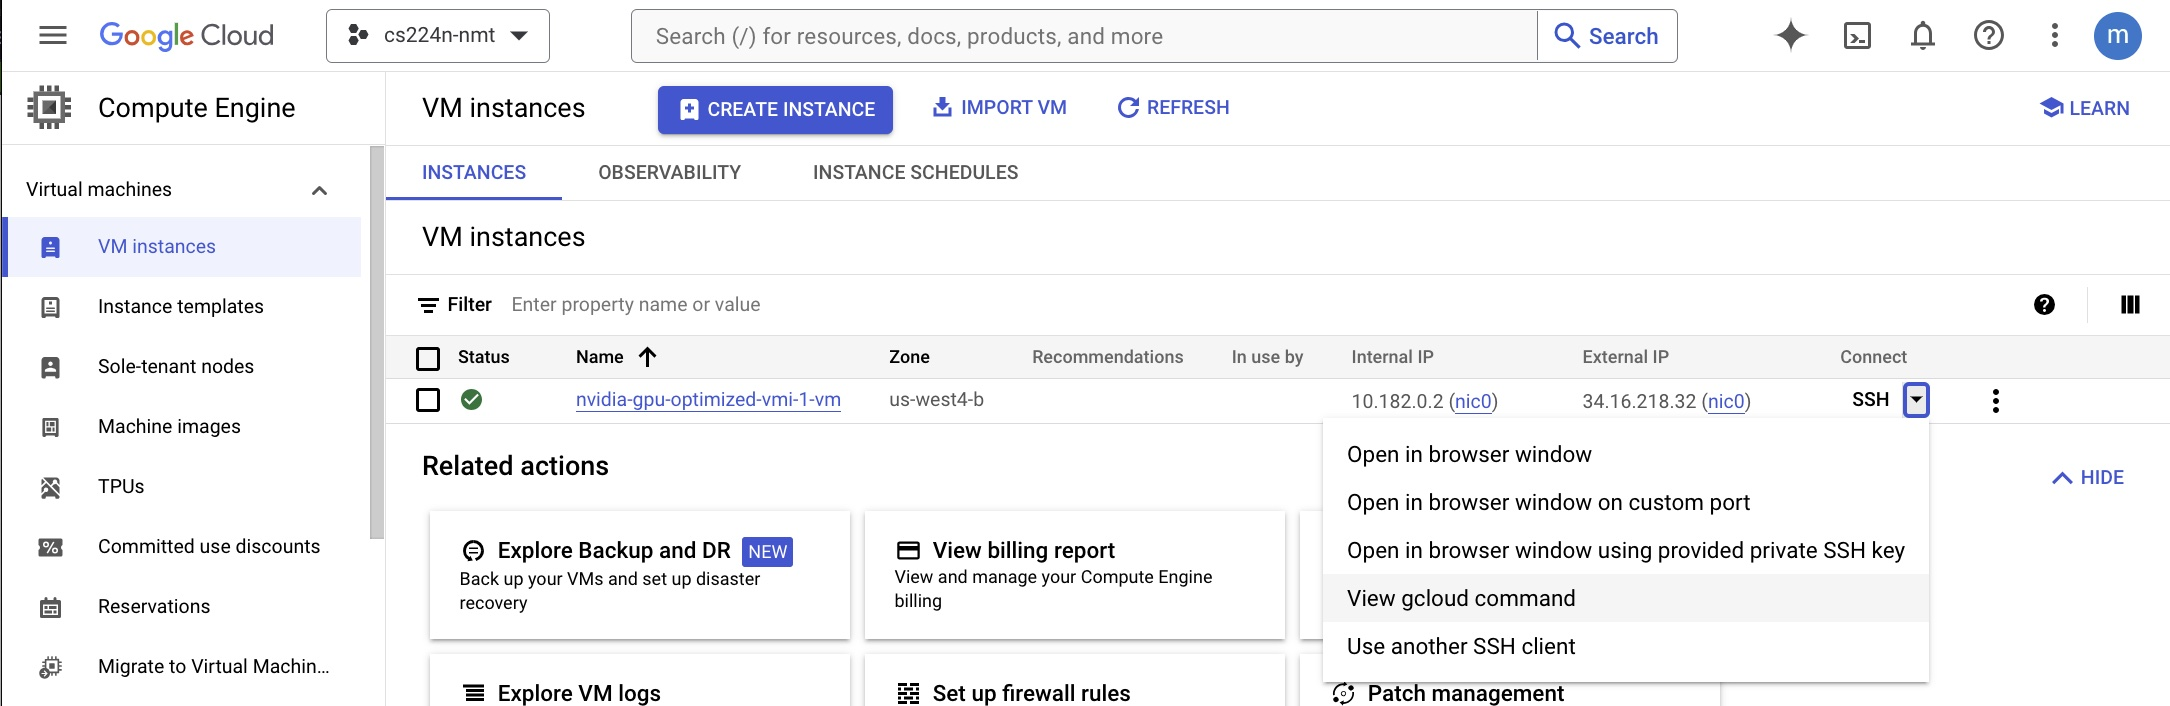
\includegraphics[width=\textwidth]{images/gcloud-dashboard.jpg}
    \caption{The cloud VM you create should be based on the \href{https://console.cloud.google.com/marketplace/product/nvidia-ngc-public/nvidia-gpu-optimized-vmi}{nvidia-gpu-optimized-vmi} virtual machine image (VMI). After deploying the instance, click on the menu near SSH and select \emph{View gcloud command} to obtain the SSH connection information.}
    \label{fig:gcloud-compute-dashboard}
\end{figure}



\paragraph{How to Connect to the Cloud VM with SSH Tunelling}
The following ssh connection command, which includes the \texttt{--ssh-flag "-L 6007:localhost:6007"} option, will also forward port 6007 of the cloud machine to the same port number on your local machine (ssh tunneling). Therefore, if the tensorboard server is running on the cloud VM and listening to port 6007, after establishing an ssh connection as follows, you will be able to access at \href{http://localhost:6007/}{http://localhost:6007/} in a web browser on your local machine.
Run the following ssh command to connect to the cloud machine. \textbf{be sure to use your own zone, project name and machine name}

\begin{lstlisting}[
    breaklines=true,
    postbreak=\mbox{\textcolor{red}{$\hookrightarrow$}\space},
]
gcloud compute ssh --zone "us-west4-b" "nvidia-gpu-optimized-vmi-1-vm" --project "grand-hangar-420500" --ssh-flag "-L 6007:localhost:6007"
\end{lstlisting}



\paragraph{How to Copy Your Code From Your Computer to the Cloud VM}
\begin{itemize}
    \item zip current directory, which should contain the \texttt{env-cpu.yml} and \texttt{env-gpu.yml} files.
\begin{lstlisting}[
    breaklines=true,
    postbreak=\mbox{\textcolor{red}{$\hookrightarrow$}\space},
]
zip -r student.zip *
\end{lstlisting}
    
    \item copy the obtained zip file to the cloud machine
\begin{lstlisting}[
    breaklines=true,
    postbreak=\mbox{\textcolor{red}{$\hookrightarrow$}\space},
]
gcloud compute scp student.zip  nvidia-gpu-optimized-vmi-1-vm:~/  --zone "us-west4-b" --project "grand-hangar-420500" 
\end{lstlisting}

\end{itemize}



\paragraph{How to Train the NMT System on the Cloud VM}
\begin{itemize}
\item If zip is not installed on your cloud machine. Install it as follows and try again.
\begin{lstlisting}[
    breaklines=true,
    postbreak=\mbox{\textcolor{red}{$\hookrightarrow$}\space},
]
sudo apt-get install zip
\end{lstlisting}

    \item Unzip student folder on the cloud machine
\begin{lstlisting}[
    breaklines=true,
    postbreak=\mbox{\textcolor{red}{$\hookrightarrow$}\space},
]
unzip student.zip -d student
cd student
\end{lstlisting}

    \item Create conda GPU environment
\begin{lstlisting}
conda env create --file env-gpu.yml
\end{lstlisting}

    \item Activate conda GPU environment
\begin{lstlisting}
conda activate cs224n-nmt-gpu    
\end{lstlisting}

    \item create a tmux session in which you start training the machine translation model
    
\begin{lstlisting}
tmux new -s s-nmt

# start the training (in the tmux session)
sh run.sh train

# detach from the tmux session
CTRL+B D
\end{lstlisting}

    \item create a tmux session in which you start TensorBoard

\begin{lstlisting}
tmux new -s s-tboard

# start the tensorboard (in the tmux session)
tensorboard --logdir runs/ --port 6007

# detach from the tmux session
CTRL+B D
\end{lstlisting}

    \item You can attach/detach from the two tmux sessions as needed. See the appendix on Tmux for basic use cases.
    \item If you established the SSH connection with the appropriate port forwarding options, you can view tensorboard in a web browser on your local machine at this address  \href{http://localhost:6007/}{http://localhost:6007/} (Fig. \ref{fig:tensorboard-gpu})

    \item when the training is complete, run the test phase

\begin{lstlisting}
tmux attach -t s-nmt
sh run.sh test
\end{lstlisting}

    \item The next section shows how to make a grade scope submission with the artifacts generated on the cloud VM.
\end{itemize}




\begin{figure}[h]
    \centering
    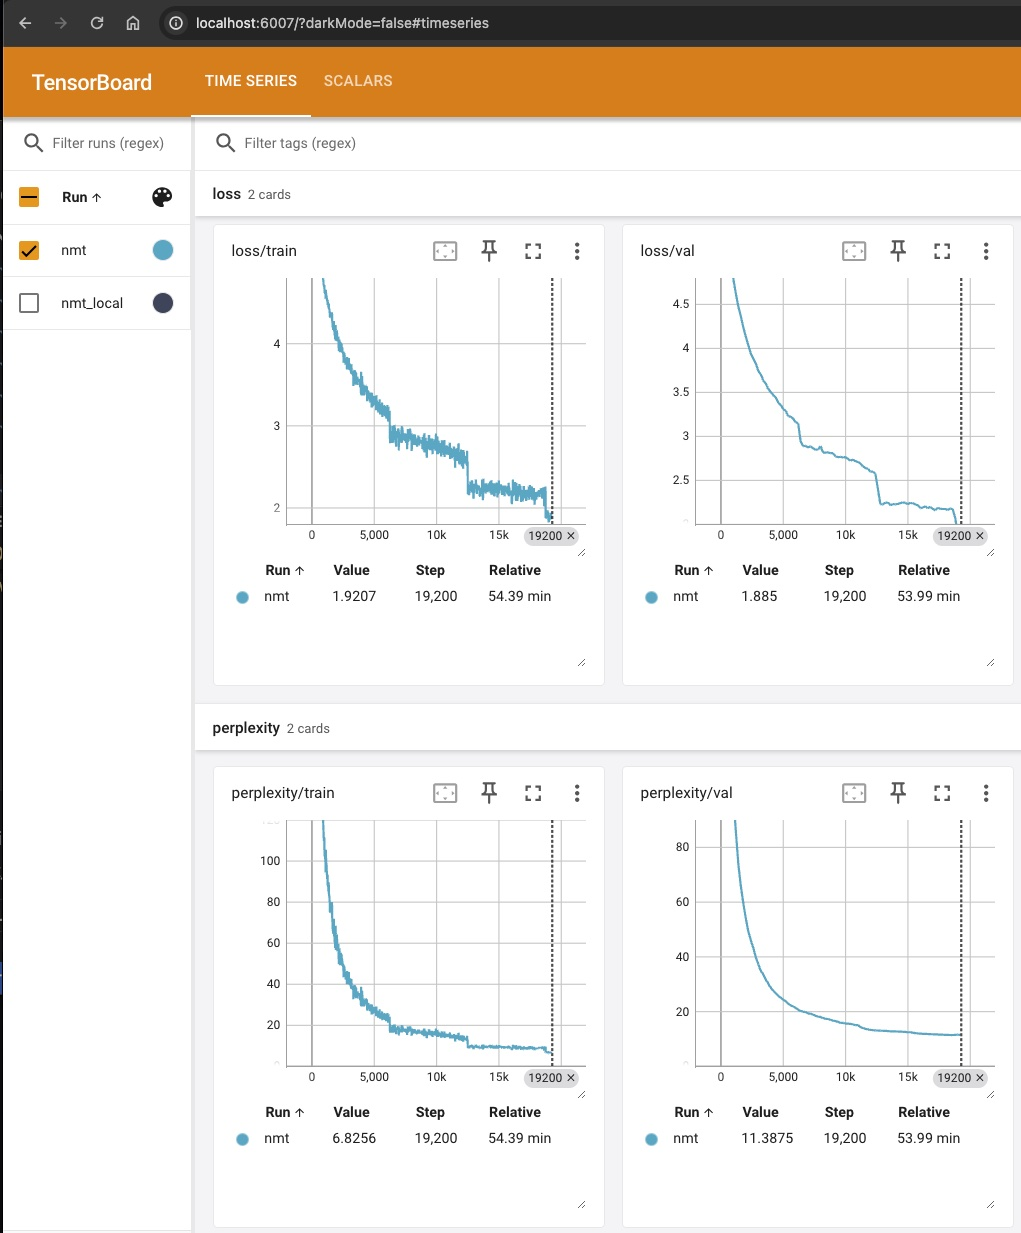
\includegraphics[height=8cm]{images/tensorboard_gpu.jpg}
    \caption{Tensorboard running on your local machine and showing loss and perplexity values on your cloud virtual machine.}
    \label{fig:tensorboard-gpu}
\end{figure}




\paragraph{How to Download the Gradescope Submission Package from Your Cloud VM}
\begin{itemize}
    \item Connect to the cloud VM as specified above
    \item On the Cloud VM, run the following command to create the gradescope submission package (\texttt{assignment3.zip})
\begin{lstlisting}[
    breaklines=true,
    postbreak=\mbox{\textcolor{red}{$\hookrightarrow$}\space},
]
sh collect_submission.sh 
\end{lstlisting}

    \item Disconnect from the cloud VM (by running \textbf{exit}), or open a terminal on your local machine. 
    \item Download the GradeScope submission package to your local machine
\begin{lstlisting}[
    breaklines=true,
    postbreak=\mbox{\textcolor{red}{$\hookrightarrow$}\space},
]
gcloud compute scp nvidia-gpu-optimized-vmi-1-vm:~/student/assignment3.zip . --zone "us-west4-b" --project "grand-hangar-420500"
\end{lstlisting}

    \item Submit  \texttt{assignment3.zip} to GradeScope
\end{itemize}

\newpage
\clearpage
\Large{\textbf{Appendix: Tmux How-to}}\\
\normalsize
\texttt{tmux} (terminal multiplexer) is a tool that lets you create and toggle between multiple terminals that run in the background, and keep then running even after you disconnect your ssh session.
%
The following assumes that you are already connected (via ssh) to your cloud virtual machine instance, and shows you basic use cases of tmux. Learn more about tmux at \href{https://github.com/tmux/tmux/wiki}{https://github.com/tmux/tmux/wiki}

\begin{itemize}
    \item  Create and attach to a new tmux session (named \emph{s-tboard})
\begin{lstlisting}
tmux new -s s-tboard
\end{lstlisting}
    \item Run a program in the new session. We will run tensorboard
\begin{lstlisting}
tensorboard --logdir runs/ --port 6007
\end{lstlisting}

\item (From within the tmux session), Detach from a tmux session, and leave the program you started running in the session.
\begin{lstlisting}
CTRL+b d
\end{lstlisting}

\item (After detaching from tmux), view all tmux sessions 
\begin{lstlisting}
tmux ls
\end{lstlisting}


\item attach to a particular tmux session (named s-nmt)
\begin{lstlisting}
tmux attach -t s-nmt
\end{lstlisting}

\item to terminate a tmux session (from within the session)
\begin{lstlisting}
exit
\end{lstlisting}

\end{itemize}


\end{document}
